\chapter{Entwurf von FLASH}
\label{chap:entwurf}
Bevor mit der Implementierung angefangen werden kann, müssen erst Entscheidungen
getroffen werden, wie die einzelnen Anforderungen umgesetzt werden sollen. Es folgt eine
schrittweise Analyse der einzelnen Anforderungen.


\begin{figure}[h]
	\centering
	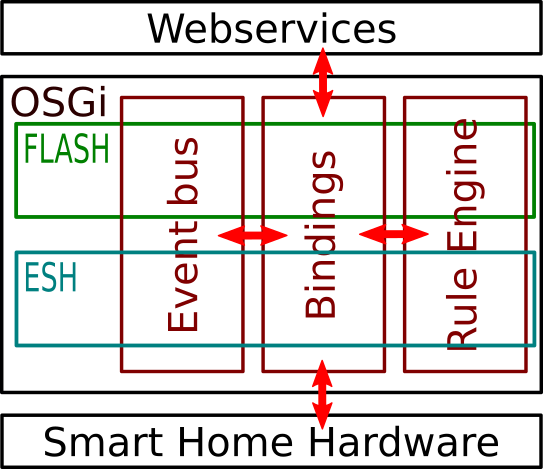
\includegraphics{bilder/entwurf_comp}
	\caption{Komponentenmodell: OSGi, ESH und FLASH}
	\label{fig:comp}
\end{figure}


\section{Überblick}
Im Rahmen der Arbeit müssen die Anforderungen umgesetzt werden, die in Sektion \ref{sec:anforderungen} zusammengefasst wurden. Durch die Nutzung von Eclipse SmartHome ist die Anforderung, dass das System in der Lage ist Geräte innerhalb des Hauses ohne Internetverbindung zu steuern, bereits gegeben. Es ist jedoch darauf zu achten, dass durch die Integration der neuen Funktionalitäten die existierenden nicht beeinträchtigt werden.\\

Einen Überblick über die verschiedenen Komponenten bietet Abbildung \ref{fig:comp}. Wie zu sehen ist, laufen sämtliche Elemente in der OSGi Umgebung. FLASH orientiert sich dabei an ESH und nutzt dieselben Ressourcen und Schnittstellen. Die zentrale Verbindungsstelle zwischen der Anwendung und den externen Funktionalitäten sind die Bindings. Sie wiederum kommunizieren mit den anderen von OSGi verwalteten Services. Der Event Bus und die Regelmaschine gehören zu den für diese Arbeit wichtigsten Diensten. ESH bietet die Interaktion mit den üblichen intelligenten Geräten in einem Smart Home (Dimmer, Jalousien, etc.), während FLASH für die Integration von den Webservices verantwortlich ist.\\


Auf welche Weise die übrigen Anforderungen umgesetzt werden sollen, wird in den nachfolgenden Sektionen diskutiert.


\section{Webservices}
Es wird im Rahmen dieser Arbeit an dieser Stelle zwischen \textit{individuellen} und \textit{gemeinsamen} Webservices unterschieden. Der wesentliche Unterschied ist, dass bei gemeinsamen Diensten keine Authentifizierung benötigt wird - sämtliche Schnittstellen und bereitgestellten Informationen sind frei verfügbar. Ein Beispiel für einen gemeinsamen Webservice kann ein online Wetterdienst sein. 

Unter individuellen Webservices handelt es sich in diesem Kontext um Dienste, deren Funktionalität vom eingeloggten User abhängt. Ein Beispiel hierfür ist \textit{Dropbox}. Der Zugriff auf die in der Dropbox gelagerten Dateien ist erst möglich, nachdem sich der User im System authentifiziert hat. 

Es gibt eine Vielzahl von verschiedenen Sicherheitsprotokollen, die an dieser Stelle zum Einsatz kommen. Vor allem hat sich derzeit der OAuth Standard etabliert, welcher auch in den Webservices \textit{Twitter} und \textit{Dropbox} genutzt wird.\\

\subsubsection{OAuth 2 Standard}
\label{subsubsec:oauth}
OAuth \cite{oauth} ist ein offener Standard für Authentifizierung, der es ermöglicht Nutzern Applikationen von Drittanbietern den (zumeist eingeschränkten) Zugriff auf Webdienste in ihrem Namen zu gestatten, ohne dabei das eigene Passwort freizugeben. Dies geschieht in der Regel in mehreren Schritten.

\begin{enumerate}
\item Die Applikation registriert sich bei dem Webservice und erhält einen Consumer-Key und Consumer-Secret.
\item Ein Nutzer möchte der Applikation gestatten auf seinen Account zuzugreifen.
\item Die Applikation teilt dem Nutzer eine URL mit, über die er dies erlauben kann. Diese URL wird vom Webservice basierend auf dem Consumer-Key bereitgestellt. 
\item Der Nutzer autorisiert sich unter der URL beim Webservice klassischerweise mit seinem Namen und Passwort. Daraufhin erhält er die Möglichkeit, der Applikation die geforderten Zugriffsrechte einzugestehen.
\item Nachdem der Nutzer die Erlaubnis erteilt hat, erhält er eine PIN, die er manuell in der Applikation eingeben muss. 
\item Nachdem er dies getan hat erhält die Applikation ein generiertes OAuth-Token, mit dem sie Zugriff auf den Account des Users hat. Der Authentifizierungsprozess ist damit abgeschlossen.
\end{enumerate}


Im Rahmen dieser Arbeit wird es nötig sein, sowohl mit gemeinsamen, als auch mit individuellen Webservices Kontakt aufzunehmen. Es wird also notwendig sein, sich gegenüber den Diensten zu authentifizieren um die erforderlichen Rechte zu erhalten, die es ermöglichen den Workflow des Nutzers zu automatisieren. Die Authentifizierung wird über die Benutzeroberfläche stattfinden.



\section{Integration in Eclipse SmartHome}
\label{sec:integrationESH}
Im Rahmen der Arbeit sollen die bereits existierenden Funktionalitäten von ESH sofern möglich wiederverwendet werden. Hierzu sollen die einzelnen Webservices durch Bindings in das System integriert werden. 
Dabei soll jede Instanz eines Webdienstes als ein Thing repräsentiert werden. Das bedeutet, dass beispielsweise im Falle eines Wetterdienstes für jeden Ort eine eigene Instanz des Thing-Typen erstellt wird, die diesen Ort darstellt. Alternativ könnte es sich bei den Instanzen um verschiedene Twitter-Accounts handeln.

Die benötigten Zugriffsdaten (z. B. OAuth-Token) werden in den Konfigurationen der Things abgelegt. Ein solcher Aufbau garantiert, dass jedes Thing über sämtliche Informationen verfügt, die benötigt werden, um es zu steuern. Die konkreten Funktionalitäten werden über ein oder mehrere Channels dargestellt. Im Rahmen dieser Arbeit wird im Demonstrator keine Nutzerverwaltung eingebaut.


\subsection{Verbindung zum Webdienst}
Nachdem ein Thing mit den benötigten Zugriffsdaten angelegt wurde, muss es vom System verwaltet werden können. Hierzu gehört vor allem die virtuelle Abbildung des realen Zustandes zu aktualisieren, sowie die tatsächliche Steuerung zu ermöglichen. 

\subsubsection{Polling und Webhooks}
Die Aktualisierung des Zustandes kann auf zwei Arten geschehen: Polling und WebHooks. Beim Polling ist die Applikation selbst dafür verantwortlich die aktuellen Werte abzurufen. Beispielsweise könnte die Applikation in einem festgelegten Intervall prüfen, welche Dateien in der Dropbox vorhanden sind. Änderungen würden in entsprechenden Events publiziert werden.\\

Falls der Webservice es unterstützt, können statt Polling auch WebHooks angewendet werden. Hierbei handelt es sich um HTTP Callbacks - die Applikation registriert also eine Adresse beim Dienst und relevante Informationen (Zustandsänderungen, etc.) werden von Dienst an diese Adresse kommuniziert. Dieser Aufbau hat den Vorteil, dass die Netzwerklast deutlich reduziert und gleichzeitig die Reaktionszeit merklich erhöht wird. Leider unterstützen derzeit nur wenige Webservices WebHooks.

\subsubsection{Verbindung}
Es soll für jedes (Webservice-)Thing, welches im System registriert wird, eine Verbindung aufgebaut werden, die auf eine der oben beschriebenen Arten die Zustände aktuell hält. Diese Verbindung soll automatisch geöffnet werden, wenn ein Gerät dem System hinzugefügt wird und wieder geschlossen werden, wenn es entfernt wird. Sie ist dafür verantwortlich bei Zustandsänderungen entsprechende Events im System zu publizieren. Die Details sollen hierbei im Payload im JSON Format bereitgestellt werden.\\

JSON wurde an dieser Stelle ausgewählt, da es die Möglichkeit bietet, komplexe Datenstrukturen über das Payload Attribut zu vermitteln. Dies erlaubt es zu vermeiden, dass jedes Binding eigene Events definieren und registrieren muss. Außerdem müssen auch die verschiedenen Handler nicht für jeden neuen Event-Typ angepasst werden - es reicht, wenn sie im Payload nach den für sie relevanten Attributen suchen. Eine Tabelle mit den publizierten Events, sowie den Eingaben und Ausgaben von Regel-Modulen ist in Abbildung \ref{table:io} aufgeführt.



\subsubsection{Eigene Events und Module von Regeln}
ESH bietet die Möglichkeit eigene Event-Typen zu definieren. Dies ist stets eine Option, die jedem Binding offen ist. Im Rahmen der Arbeit reicht es jedoch, einen allgemeinen neuen Event-Typ zu definieren und daraufhin die konkreten \textit{topics} und \textit{payloads} zu variieren. Beispielsweise würde bei Hochladen einer neuen Datei in die Dropbox ein Event mit dem Topic \glqq flash/dropbox/added\grqq{} und einem Payload, dass die Metadaten (Name, Pfad, etc.) der Datei im JSON Format enthält, im System publiziert.\\

Analog soll mit Triggern, Conditions und Actions von Regeln umgegangen werden. Es sollen zunächst \textit{GenericEventTrigger} und \textit{EventCondition} zum Einsatz kommen. 

Der \textit{GenericEventTrigger} ist ein von ESH bereits implementierter Auslöser, der die Ausführung einer Regel anstoßt, wenn ein Event eintrifft. Das erwartete Event kann vom Nutzer konfiguriert werden. Der Trigger stellt das auslösende Event außerdem im Kontext (siehe Sektion \ref{subsubsec:kontext}) bereit.

Die \textit{EventCondition} ermöglicht es das erhaltene Event nach seinen Attributen zu filtern. In der Konfiguration der Bedingung werden reguläre Ausdrücke für die vier Attribute des Events hinterlegt. Wenn die Bedingung evaluiert wird, wird geprüft, ob die tatsächlichen Werte des Events mit dem Regex übereinstimmen. 

Zusammen decken diese beiden Module einen großen Teil der möglichen Szenarien ab. Bindings, die Funktionalitäten anbieten oder einer Logik bedürfen, die von diesen Werkzeugen nicht abgedeckt werden kann, haben stets die Option eigene Module im System zu registrieren.




\subsection{Persistenz}
Wie in Sektion \ref{subsec:persistenz} erläutert, ist eine MapDB in ESH bereits integriert. Da im Rahmen dieser Arbeit die Menge an persistierten Daten sich nicht maßgeblich verändern wird, ist es nicht notwendig, auf eine mächtigere Datenbank umzusteigen. 
%Da im Rahmen dieser Arbeit nur geringe Mengen an Daten persistiert werden müssen, ist es nicht notwendig, auf eine mächtigere Datenbank umzusteigen. 

Dadurch, dass die Webservices selbst als Things modelliert werden und alle notwendigen Konfigurationsdaten mit sich tragen, kann dieser Aspekt von ESH in seiner aktuellen Form wiederverwendet werden. Bei einem Neustart des Systems werden sämtliche relevante Things aus der Datenbank ausgelesen und basierend auf den in ihrer Konfiguration gespeicherten Zugriffsdaten (z. B. OAuth Token) entsprechende Verbindungen aufgebaut, die für die Aktualität der Zustände sorgen.

\subsection{Benutzeroberfläche}
\label{entwurf:gui}
\subsubsection{Funktionale Anforderungen}
Die Benutzeroberfläche soll den Nutzer in die Lage versetzen Regeln zur Laufzeit zu bearbeiten. Das bedeutet, es soll ihm möglich sein neue Regeln anzulegen, sowie existierende Regeln zu betrachten, zu editieren und zu löschen. Da Eclipse SmartHome die Möglichkeit bietet Regeln im JSON-Format zu deklarieren (siehe Sektion \ref{subsec:decltypes}), bietet es sich an dieser Stelle an, es in der Benutzeroberfläche analog umzusetzen.\\

Des Weiteren soll dem User die Möglichkeit gegeben sein, die Zugriffsrechte auf die unterstützten Webservices (z. B. auf seinen Twitter Account) der Anwendung zu übermitteln, bzw. auf diese Weise neue Instanzen des entsprechenden Thing-Typen zum System hinzuzufügen.

\subsubsection{Umsetzungskonzept}
Die zu entwickelnde grafische Benutzeroberfläche soll modernen Design-Prinzipien entsprechen. Im Rahmen dieser Arbeit wurde entschieden diese in Form einer Einzelseiten-Webanwendung zu realisieren. \\

Das Format einer \textit{Web}-Anwendung bietet sich an, da es dem Nutzer möglich sein soll seine angebundenen Geräte von überall steuern zu können. Eine Anwendung, die nativ auf dem Raspberry Pi arbeitet und nur verwendet werden kann, sofern man physischen Zugriff auf das Gerät hat, würde am Ziel vorbei führen. Im Umfeld von Smart Home sind Webanwendungen seit langem zum Standard geworden.\\

Es soll sich dabei um eine \textit{Einzelseiten}-Webanwendung (engl. Single Page Application (SPA))handeln, da sie sich gut für dieses konkrete Szenario eignet. Bei einer SPA handelt es sich um ein Design Paradigma, bei dem die gesamte Anwendung auf einer einzigen HTML-Seite entwickelt wird \cite{gui_sp}. Inhalte werden dynamisch vom Server angefragt, wenn sie benötigt werden und auf der Seite angemessen präsentiert. In der Regel kommt dabei vor allem asynchroner Javascript zum Einsatz.

Einzelseiten-Webanwendungen eignen sich gut für die im Rahmen dieser Arbeit behandelte Problemstellung, da sie es ermöglichen die Belastung auf den Server zu reduzieren. Dies ist wichtig, da die Rechenleistung eines Raspberry Pi vergleichsweise begrenzt ist und eine Server seitige Bearbeitung und Bereitstellung von HTML-Inhalten zu Verzögerungen führen könnte.\\

Seitens des Servers sollen die Informationen über REST Schnittstellen \cite{rest} bereitgestellt werden. Es wurde entschieden für die  Kommunikation Representational State Transfer zu wählen, da es aktuell als Referenz-Paradigma für die Bereitstellung von intelligenten Geräten im Web gilt \cite{gui_rest}.



\section{OSGi auf dem Raspberry Pi}
\label{sec:deploy}
Eclipse SmartHome besteht aus einer Reihe von OSGi Bundles und die im Rahmen der Arbeit erstellten zusätzlichen Funktionalitäten nehmen ebenfalls diese Form an. Es lässt sich annehmen, dass sofern ein OSGi Container auf dem Pi laufen wird, auch das gesamte Framework gestartet werden kann.\\

Konkret betrachtet wird auf dem Raspberry Pi ein Betriebssystem benötigt, das Java unterstützt. Daraufhin muss ein OSGi Container wie beispielsweise Concierge\cite{concierge} oder Apache Felix GoGo\cite{felixgogo} gestartet werden. Danach muss er entsprechend konfiguriert werden, sodass die Jar-Dateien der relevanten ESH Bundles auf die benötigten allgemeinen System-Jars von Java Zugriff haben. Schließlich müssen alle Abhängigkeiten der im Container installierten Bundles erfüllt sein, damit sie gestartet werden können. Beispielsweise bedarf eine Web-UI eines entsprechenden HTTP Servers.


\section{Fazit}
Jeder Webdienst wird in einem eigenen Binding in das System integriert. Dabei werden Thing-Typen registriert, deren Instanzen konkrete Ausprägungen des Webservices repräsentieren. Für jede Thing-Instanz wird eine Verbindung aufgebaut, die für die Aktualität der Zustandsdaten und das Publizieren entsprechender Events verantwortlich ist. Jedes Binding entscheidet selbst, ob ihm die existierenden Module ausreichen oder es neue Entitäten im System registriert. 






